\documentclass[a4paper,11pt]{report}
\usepackage[left=3cm, right=3cm, top=3cm, bottom=3cm]{geometry}
\usepackage{graphicx}
\usepackage{listings}
\usepackage{titlesec}
\usepackage{fancyhdr}
\usepackage{epstopdf}
\usepackage{float}
\usepackage{amsmath}
\usepackage{setspace}
\usepackage{eufrak}
\usepackage{url}
\usepackage{listings}
\usepackage{courier}
\usepackage{hyperref}
 \newcommand{\textform}[1]{\fontsize{14}{20}\selectfont{#1}}
\pagestyle{fancy}
\fancyhf{}
\fancyhead[R]{\thepage}
\renewcommand{\chaptermark}[1]{\markboth{#1}{}}
\renewcommand{\headrulewidth}{1pt}
\renewcommand{\footrulewidth}{1pt}

\lhead{\footnotesize{JOBCONNECT}}
\rhead{}
\lfoot{\footnotesize{Department of Computer Science \& Engg.}}
\cfoot{}
\rfoot{\thepage}

\titleformat{\chapter}[display]
{\normalfont\Large\bfseries\centering}{\chaptertitlename\
\thechapter}{20pt}{\Large}

\begin{document}

\thispagestyle{empty}
  \begin{center}
      \fontsize{22}{25}\selectfont{\textbf{GOVERNMENT POLYTECHNIC COLLEGE PERUMBAVOOR}}\\[.1cm]
            \fontsize{15}{25}\selectfont{\textbf{Koovappady P.O Ernakulam-683 544 Kerala
    }}\\[1.2cm]
\begin{figure}[h]
	\centering
	\hspace{21pt}
	
\includegraphics[width=.50\linewidth]{logo.png}
	\label{fig:logo.png}
\end{figure}

\fontsize{14}{25}\selectfont{\textbf{Computer Engineering 2022-23}}\\
\fontsize{14}{25}\selectfont{\textbf{Semester IV}}\\[1cm]

\fontsize{14}{25}\selectfont{\textbf{PROJECT REPORT}}\\[.1cm]
    \fontsize{14}{25}\selectfont{on}\\
    \fontsize{20}{25}\selectfont{\textbf{JOBCONNECT}}\\[.1cm]
    \fontsize{14}{25}\selectfont{\textbf{A JOB SEARCHING APPLICATION}}\\[1.2cm]
    \fontsize{12}{25}\selectfont{\textbf{Submitted by}}\\[.2cm]
    \fontsize{14}{25}\selectfont \bfseries{SREEKUMAR P UNNIKRISHNAN} \\ \fontsize{12}{25}\selectfont{\textbf{20130126}} \\

    
%\vfill
 \end{center}

\fontsize{12pt}{20}\selectfont
\thispagestyle{empty}


\newpage
  \thispagestyle{empty}

    \begin{center}
      \fontsize{14}{20}\selectfont \textbf{GOVERNMENT POLYTECHNIC COLLEGE PERUMBAVOOR}\\
     
    \fontsize{14}{20}\selectfont \textbf{
DEPARTMENT OF COMPUTER ENGINEERING}\\[1.5cm]
\begin{figure}[h]
\centering
	\hspace{.5cm}

\includegraphics[width=0.3\linewidth]{logo.png}
	\label{fig:logo.png}
\end{figure}

     
      \textbf{CERTIFICATE}
    \end{center}
    \vspace{.5cm}
    \textform{This is to certify that the project report entitled \textbf{JobConnect - A Job Searching Application} submitted by \textbf{Sreekumar P Unnikrishnan} is approved for submission requirement for 6009 -Project and Seminar in  $6^{th}$ semester Computer Engineering at Govt.Polytechnic College,Perumbavoor.}\\[0.15cm]


\begin{minipage}{.40\textwidth}
    \begin{flushleft}
        \begin{center}
            \fontsize{12}{25}\selectfont{\textbf{Head of Section}}\\[1.5cm] 
        \end{center}
    \end{flushleft}
\end{minipage}
\hfill
\begin{minipage}{0.40\textwidth}
    \begin{flushright}
        \begin{center}
            \fontsize{12}{25}\selectfont{\textbf{Lecturer in Charge}}\\[1.5cm]
        \end{center}
    \end{flushright}
\end{minipage}




\vspace{1cm}
\begin{flushleft}
  \fontsize{12}{20}\selectfont \textbf{Date  :}\\
  \fontsize{12}{20}\selectfont \textbf{Place :}
\end{flushleft}
\vspace{1cm}
\begin{minipage}{.4\textwidth}
    \begin{flushleft}
    \begin{center}
    
    \fontsize{14}{25}\selectfont \bfseries{Internal Examiner}\\[.1cm]
    
%\vfill
 \end{center}
    \end{flushleft}
      \end{minipage}
\begin{minipage}{0.8\textwidth}
\begin{flushright}
\begin{center}
 
%\vfill
\fontsize{14}{25}\selectfont \bfseries{External Examiner}\\[.1cm]

\end{center}
\end{flushright}
\end{minipage}


\newpage
\fontsize{12pt}{20}\selectfont
\thispagestyle{empty}
  \renewcommand\abstractname{\textform{\textbf{ACKNOWLEDGMENT}}}
    \begin{abstract}
      \vspace{2.5cm}
      
         I would like to express my sincere gratitude to all those who have contributed to the successful completion of my project JobConnect - The Job Searching Application. This opportunity has allowed me to delve into a fascinating field of web development and expand my knowledge in computer engineering.

First and foremost, I extend my heartfelt appreciation to Dr. Aiju Thomas, the Principal of Government Polytechnic College Perumbavoor. I am grateful for his constant support, guidance, and encouragement throughout my academic journey. His visionary leadership and commitment to excellence have created an environment conducive to learning and exploration.

I am indebted to Mr. Biju Peter, the Head of the Department of Computer Engineering, for his invaluable guidance and mentorship. His expertise, patience, and enthusiasm have been instrumental in shaping my understanding of the subject and honing my research skills. I am thankful for his unwavering support and valuable insights that have enriched my project.

I would also like to acknowledge the faculty members of the Computer Engineering Department for their constant support and encouragement throughout my academic journey. Their expertise and passion for teaching have played a significant role in shaping my intellectual growth.

I would like to express my gratitude to my classmates and team members for their support and encouragement. Their presence and collaboration have made the learning experience enjoyable and memorable.

Thank you all for your unwavering support and belief in me.
    \end{abstract}
 
  \tableofcontents
\thispagestyle{empty}

\chapter{Introduction}

\paragraph{}The JobConnect project is an online platform designed to connect job seekers with employers, aiming
to streamline the job search and recruitment process. In today's competitive job market, both job seekers and employers face challenges in finding the right match for their needs. The Job Junction
platform seeks to bridge this gap by providing a centralized platform where job seekers can explore job
opportunities and employers can efficiently manage the hiring process.


The primary goal of Job Junction is to provide a user-friendly interface that simplifies the job search
experience for candidates. With an intuitive design and advanced search functionality, job seekers can
easily browse and apply for relevant job openings based on their preferences, including location,
industry, experience level, and more. 

The implementation of the Job Junction platform involves utilizing modern web development
technologies and databases. Front-end technologies like HTML, CSS, and JavaScript, along with
frameworks such as React or Angular, ensure a responsive and intuitive user interface. Back-end is php
utilized to handle the server-side functionality and facilitate data management. Secure user
authentication and authorization protocols, integration with third-party APIs, and a robust database
management system ensure the platform's reliability and security.


By connecting job seekers with employers, Job Junction aims to optimize the job market ecosystem,
making the job search process more efficient and effective for both parties involved. Through its
comprehensive features and user-friendly interface, the Job Junction platform strives to be a valuable
resource for job seekers and a powerful tool for employers, ultimately contributing to the success and
growth of individuals and businesses in the professional world.

  
\chapter{Lack of Efficient Job Matching}
The Job Junction project aims to address the following key problems in the job search and recruitment
process:

\section{Manual and Time-Consuming Process}
 Job seekers often struggle to find job opportunities that align with
their skills, experience, and career aspirations. Similarly, employers face challenges in identifying
qualified candidates for their job vacancies. The lack of an efficient job matching system results in timeconsuming and inefficient recruitment processes.
\section{Limited Access to Job Opportunities}
 Job seekers, particularly those in remote areas or with limited
resources, face difficulties in accessing a wide range of job opportunities. Traditional job search methods
such as newspaper listings or physical job fairs have limitations in reaching a broader audience, leaving
potential candidates unaware of available positions.
\section{Ineffective Communication and Tracking}
Employers and job seekers encounter communication
challenges during the hiring process. Lack of streamlined communication channels and effective tracking
mechanisms lead to delays, miscommunication, and the potential loss of suitable candidates.

\section{Data Security and Privacy Concerns}
In the digital age, data security and privacy are critical concerns
for both job seekers and employers. Existing job portals may not provide adequate measures to protect
user information and maintain confidentiality, making individuals hesitant to share their personal and
professional details.
\section{Complex and Non-Intuitive User Interfaces}
Many existing job portals suffer from complex and nonintuitive user interfaces, making it challenging for users to navigate the platform and utilize its features
effectively. This results in user frustration and a suboptimal user experience.

\chapter{Solutions}
To address the problems outlined in the problem statement, the Job Junction project proposes the
following solutions:

\section{Advanced Job Matching Algorithm}
 Implement an intelligent job matching algorithm that considers
job seekers' skills, experience, qualifications, and preferences, as well as employers' requirements. This
algorithm will provide more accurate and relevant job recommendations, improving the efficiency of the
job matching process.

\section{Broad Job Opportunity Reach}
 Establish partnerships with companies and organizations across various
industries to ensure a wide range of job opportunities are available on the platform. Utilize digital
marketing strategies and social media platforms to reach a larger audience, including job seekers in
remote areas or with limited resources, thereby enhancing accessibility to job opportunities.
\section{Streamlined Communication and Tracking}
 Develop a robust and user-friendly communication system
within the platform to facilitate seamless interaction between employers and job seekers. Implement
features such as in-app messaging, interview scheduling, and application status tracking, allowing both
parties to communicate effectively and track the progress of the hiring process.
\section{Data Security and Privacy Measures}
Implement stringent security measures to protect user data and
maintain privacy. Utilize encryption protocols, secure data storage practices, and regular security audits
to ensure the confidentiality and integrity of user information. Comply with relevant data protection
regulations and provide transparency regarding data handling practices to build trust among users.

\section{Intuitive User Interface Design}
Create a clean and intuitive user interface that is easy to navigate and
understand. Conduct user testing and feedback sessions to identify pain points and refine the interface
accordingly. Simplify the job search and application process, providing clear instructions and guidance to
enhance the overall user experience.
\section{ Continuous Improvement and Feedback Integration}
Regularly gather user feedback and analyze user
behavior data to identify areas for improvement. Incorporate user suggestions and make iterative
updates to enhance the platform's functionality and usability. Maintain an open line of communication
with users to address their needs and adapt to changing job market dynamics.

\chapter{Requirement Analysis}
To ensure the successful implementation of the Job Junction project, a comprehensive requirement
analysis was conducted. The following requirements were identified to meet the needs of job seekers
and employers:
\section{User Registration and Profile Creation}
\begin{itemize}
  \item Job seekers and employers should be able to create user accounts and profiles on the Job Junction
platform.
  \item User registration should require essential information such as name, email address, and password.
  \item  Job seekers should be able to provide additional details such as education, work experience, and
skills in their profiles.
	\item  Job seekers should be able to provide additional details such as education, work experience, and
skills in their profiles.
\item Employers should be able to provide information about their company, including the industry, size,
and location.
\end{itemize}

\section{Job Search and Filtering}
\begin{itemize}
  \item Job seekers should be able to search for job opportunities based on various criteria such as location,
industry, job title, and experience level.
\item - Advanced search filters should be implemented to allow job seekers to refine their search results
based on specific preferences.
\item The search functionality should provide accurate and relevant job listings that match the criteria
specified by the job seekers.
\end{itemize}

\section{Job Posting and Management}
\begin{itemize}
  \item Employers should have the ability to post job vacancies on the Job Junction platform.
  \item Job postings should include details such as job title, description, requirements, location, and
application instructions.
\item Employers should be able to manage and update their job postings, including marking positions as
filled or expired.
\end{itemize}

\section{Application Submission and Management}
\begin{itemize}
  \item  Job seekers should be able to submit their applications for job openings directly through the
platform.
  \item The application process should allow job seekers to upload their resumes/CVs and cover letters.
  \item Employers should have a dedicated interface to manage and review received applications, including
the ability to shortlist, interview, and provide feedback to candidates.
\end{itemize}

\section{Communication and Interaction}
\begin{itemize}
  \item The platform should facilitate communication between employers and job seekers.
  \item In-app messaging or chat functionality should be available for employers and job seekers to
communicate regarding job opportunities, application status, and interview scheduling.
\item Notifications and alerts should be implemented to keep users informed about application updates,
new job postings, and relevant communication.
\end{itemize}

\section{User Experience and Interface Design}
\begin{itemize}
  \item The platform should have an intuitive and user-friendly interface that is easy to navigate and
understand.
\item The design should be responsive, ensuring compatibility across different devices and screen sizes.
\item Clear instructions and guidance should be provided to assist users in using the platform effectively.
\end{itemize}
\section{Data Security and Privacy}
\begin{itemize}
\item Robust data security measures should be implemented to protect user information and maintain
privacy.
\item  User data, including personal and professional details, should be securely stored and encrypted.
\item The platform should comply with relevant data protection regulations, such as GDPR or local privacy
laws.
\end{itemize}

It is crucial to review and fulfill these system requirements to ensure a smooth setup and execution of the project. Additionally, regularly updating the dependencies and software versions as recommended by the project maintainers will help maintain compatibility and security.


\chapter{Technologies used}

The technologies used to create the project are as follows:

\section{HTML}
HTML, which stands for Hypertext Markup Language, is the standard markup language used for creating the structure and content of web pages. It provides a set of tags or elements that define the various components of a webpage, such as headings, paragraphs, images, links, tables, forms, and more.

HTML is a markup language, meaning it uses markup tags to define the structure and semantics of the content. These tags are enclosed in angle brackets (< >) and are placed within the content of a webpage to give it meaning and structure. For example, the <h1> tag is used to define the main heading of a page, while the <p> tag is used to define paragraphs.

\section{CSS}
CSS, or Cascading Style Sheets, is a powerful styling language used in web development to enhance the visual presentation of HTML documents. It provides a comprehensive set of rules and properties that enable developers to control the layout, colors, fonts, and other design aspects of a website. With CSS, designers can create engaging and attractive web pages, ensuring a consistent and professional appearance across different browsers and devices.

One of the main advantages of CSS is its ability to separate the content and structure of a web page from its visual styling. This separation allows for easy maintenance and updates, as changes can be made to the CSS file without altering the underlying HTML structure. CSS also enables efficient styling through the use of selectors, which target specific elements or groups of elements on a web page. By applying different styles to different elements, developers can achieve a customized and dynamic user interface.

\section{JavaScript}
JavaScript is a versatile programming language commonly used in web development to add interactivity and dynamic behavior to websites. It is a client-side scripting language, meaning it runs directly in the web browser of the user, enhancing the functionality and user experience of the web pages. JavaScript can be embedded within HTML documents or included in separate external files, providing flexibility and modularity in coding.

One of the key features of JavaScript is its ability to manipulate the Document Object Model (DOM). The DOM represents the structure of an HTML document, and JavaScript allows developers to access and modify this structure, making changes to elements, styles, and content dynamically. Through DOM manipulation, JavaScript enables real-time updates, interactive forms, dynamic content loading, and other engaging user interactions.

\section{PHP}
PHP (Hypertext Preprocessor) is a widely used server-side scripting language designed specifically for web development. It is a powerful and versatile language that allows developers to create dynamic and interactive web applications. PHP code is embedded within HTML documents and is executed on the server, generating dynamic content that is then sent to the user's web browser.

One of the main advantages of PHP is its ability to interact with databases. PHP supports a wide range of database management systems, including MySQL, PostgreSQL, and SQLite. This makes it easy to retrieve, store, and manipulate data from databases, enabling the creation of dynamic web pages that can handle user input, process forms, and generate personalized content.

\section{MySQL}
MySQL is an open-source relational database management system (RDBMS) that is widely used for storing and managing structured data. It is a popular choice for web applications and is known for its reliability, performance, and ease of use. MySQL is compatible with various operating systems, including Windows, Linux, and macOS, making it versatile and accessible to developers.

One of the key features of MySQL is its ability to handle large volumes of data efficiently. It provides fast and scalable database operations, allowing for quick data retrieval, storage, and modification. MySQL supports a wide range of data types, including numeric, string, date, and time, as well as more advanced types like JSON and spatial data. This flexibility enables developers to store and process diverse types of information in their applications.

\section{XAMPP}
XAMPP is a popular cross-platform software package that provides a complete web development environment. The name "XAMPP" stands for Cross-Platform (X), Apache (A), MySQL (M), PHP (P), and Perl (P), which are the key components bundled within the package. It is designed to simplify the setup and configuration of a local web server, making it easy for developers to create and test web applications on their own machines.

One of the main features of XAMPP is the Apache web server, which is a widely used server software for hosting websites and serving web content. Apache provides a reliable and efficient platform for running PHP, HTML, and other web-based technologies. With XAMPP, developers can quickly set up an Apache server environment on their local machine without the need for complex configurations.

\chapter{Code}
\section{Database connection}
PHP code to connect to database
\begin{verbatim}
$host = "localhost";
$uname = "root";
$password = "";
$db = "project";

$con = mysqli_connect($host, $uname, $password, $db);
\end{verbatim}

\section{Registration}
PHP code to insert data into the database

\begin{verbatim}
if(isset($_POST['name']) && isset($_POST['email']) &&
isset($_POST['pw']) && isset($_POST['confirm-pw'])) {
	$user = $_POST['name'];
	$email = $_POST['email'];
    $rollno = $_POST['rollno'];
	$pw = $_POST['pw'];
	$confirm_pw = $_POST['confirm-pw'];

	if ($pw == $confirm_pw) {
		$sql = "INSERT INTO studentreg (name, email, rollno, password) values 
		('$user', '$email', '$rollno', '$pw')";
		mysqli_query($con, $sql);
		echo "<script>alert('User registered successfully!');
		</script>";
	} else {
		echo "<script>alert('Passwords do not match. Please try again.');
		</script>";
	}
}
\end{verbatim}

\section{Login}
PHP code to create PHP login
\begin{verbatim}
if ($_SERVER['REQUEST_METHOD'] == 'POST'{
  $roll = $_POST['roll'];
  $password = $_POST['password'];

  $con = mysqli_connect($host, $uname, $pswd, $db);

  $valrol = "SELECT password FROM studentreg WHERE rollno = '$roll'";
  $result = mysqli_query($con, $valrol);

  $row = mysqli_fetch_assoc($result);
  $hashed_password = $row['password'];

  if ($password == $hashed_password) {
    header('Location: studentpage.php');
    exit;
	} else {
    echo '<script>alert("Incorrect password. Please try                                  again.")</script>';
	}
}
\end{verbatim}
\section{Password Validation}
Code to validate password
\begin{verbatim}

$result = mysqli_query($conn, "SELECT password FROM users 
WHERE username = '$username'");
$row = mysqli_fetch_assoc($result);
$hashed_password = $row['password'];

// Verify the password entered by the user
if (password_verify($password, $hashed_password)) {
    // Password is correct, authenticate the user
    session_start();
    $_SESSION['username'] = $username;
    header("Location: dashboard.php");
} else {
    // Password is incorrect, show an error message
    echo "Invalid username or password.";
}


\end{verbatim}

\section{Data fetch}
Code to fetch data from database and display it on table.
\begin{verbatim}
function display($result)
{
  echo "<div class='container'>";
  echo "<table class='table table-striped table-bordered table-hover'>";
  echo "<thead class='table-dark'><tr><th>Company Name</th><th>Job 
  description</th><th>District</th><th>Location</th><th>Department
  </th><th>Last Date for Regestration</th><th>Registration Link
  </th></tr></thead>";
  
  while ($row = mysqli_fetch_assoc($result)) {
      echo "<tr>";
      echo "<td>" . $row['title'] . "</td>";
      echo "<td>" . $row['descr'] . "</td>";
      echo "<td>" . $row['distr'] . "</td>";
      echo "<td>" . $row['loc'] . "</td>";
      echo "<td>" . $row['dep'] . "</td>";
      echo "<td>" . $row['date'] . "</td>";
      echo "<td><a href='" ."http://". $row['link'] . "'
      class='btn btn-primary'  target='_blank'>Register</a></td>";
      echo "</tr>";
  }
  echo "</table>";
  echo "</div>";
  
}
\end{verbatim}



\chapter{Screenshots}

\section{Home Page}
\begin{figure}[h]
	\centering
	\hspace{21pt}
	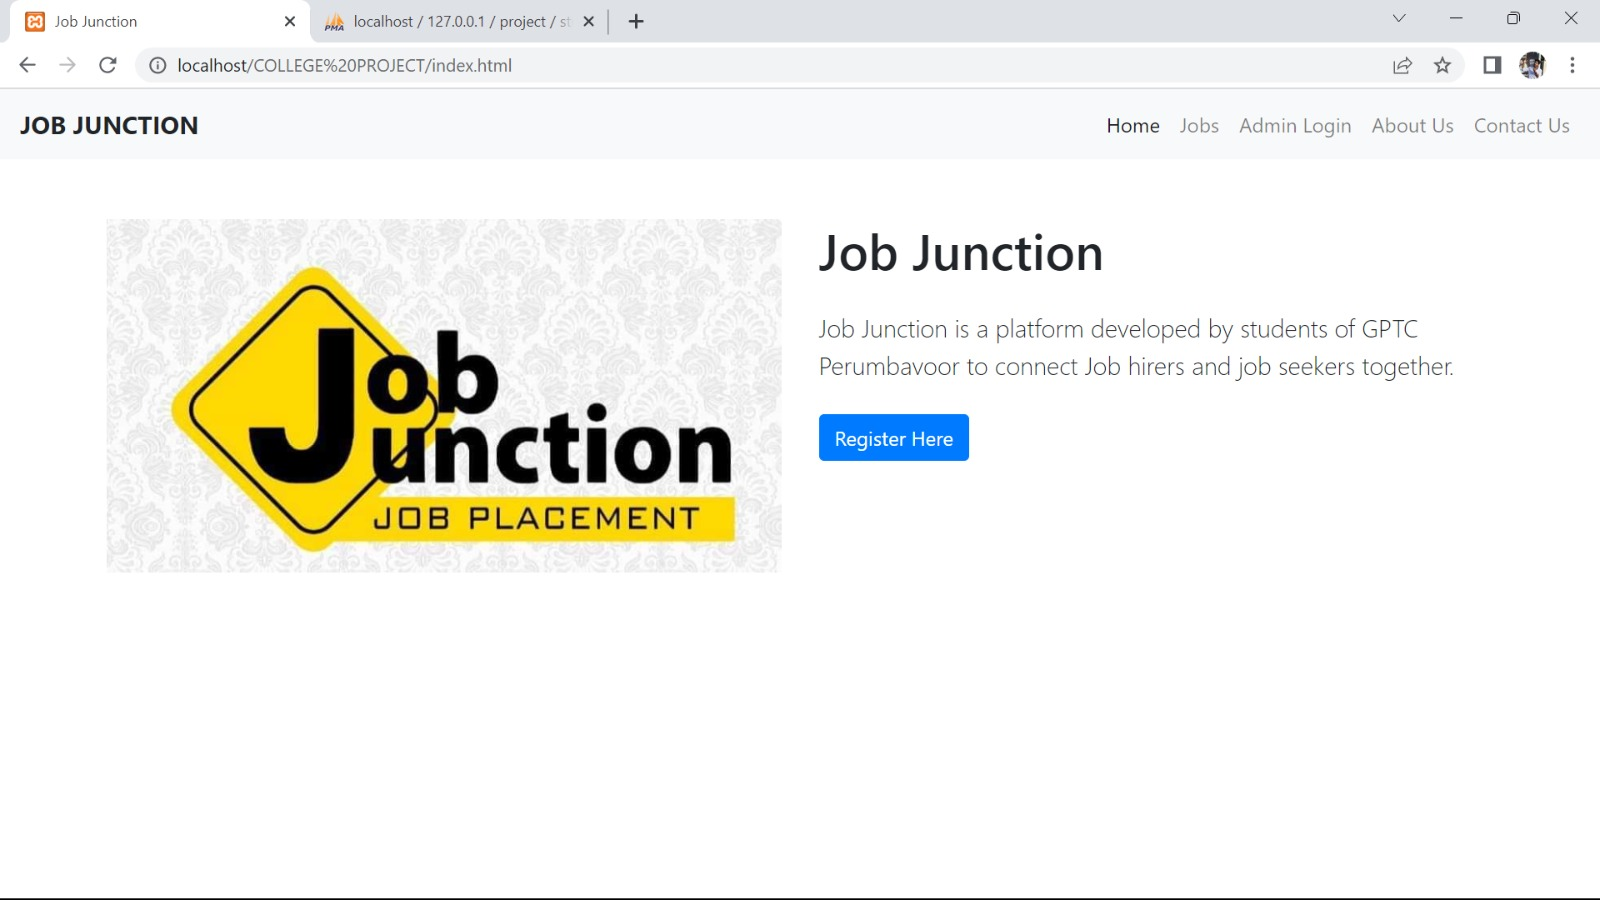
\includegraphics[width=.70\linewidth]{job10.jpeg}
	\label{fig:jop10.jpeg}
\end{figure}

\section{Login}
The users can login using id number and password.
If the department doesn't have an account, they need to sign up to use the application. 
\begin{figure}[h]
	\centering
	\hspace{21pt}
	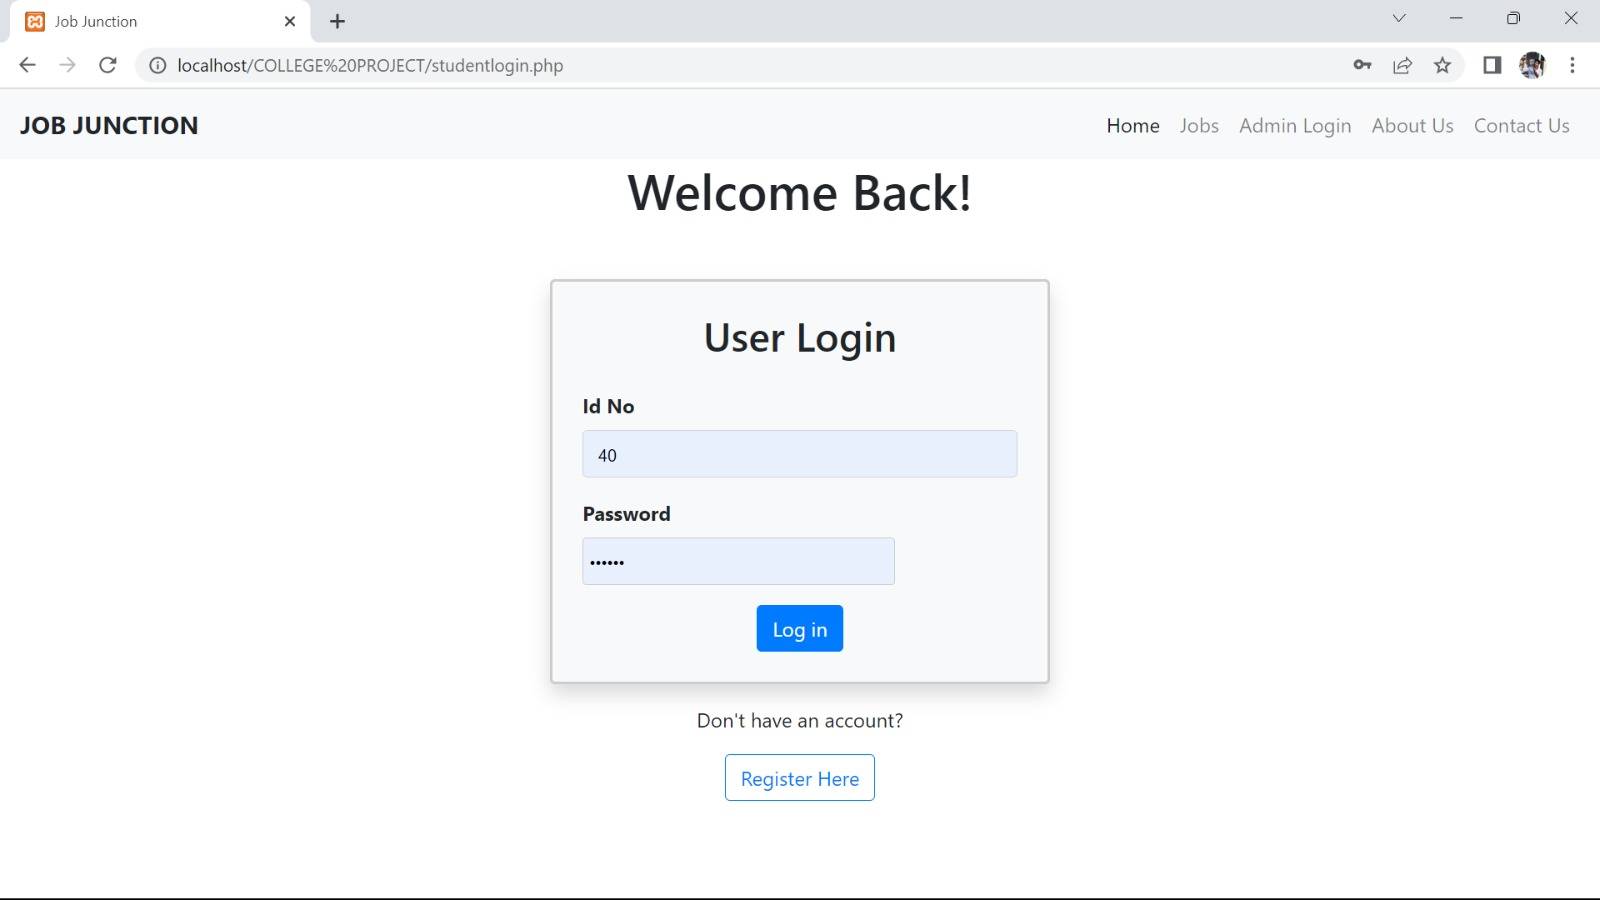
\includegraphics[width=.70\linewidth]{job5.jpeg}
	\label{fig:job5.jpeg}
\end{figure}

\section{User Registration}
If users doesn't have an account, they need to register. Departments can register using name, email and aadhar number. The already registered email and aadhar number cannot be duplicated.
\begin{figure}[h]
	\centering
	\hspace{21pt}
	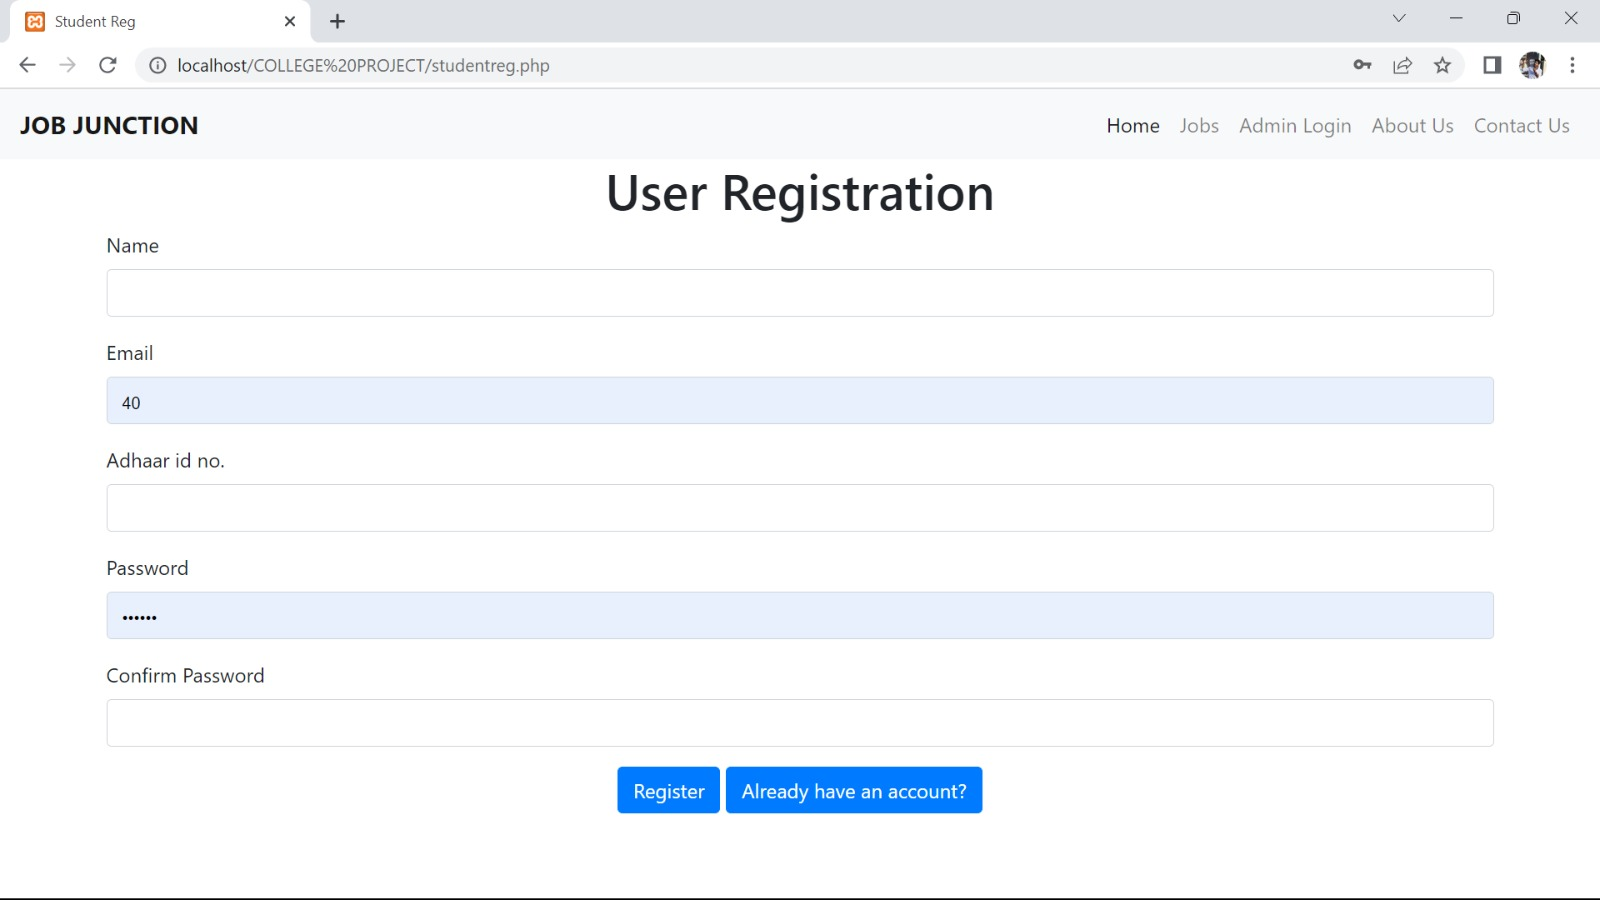
\includegraphics[width=.70\linewidth]{job4.jpeg}
	\label{fig:job4.jpeg}
\end{figure}

\section{Company Registration}
Companies can register using name, email and password. The already registered email cannot be duplicated.
\begin{figure}[h]
	\centering
	\hspace{21pt}
	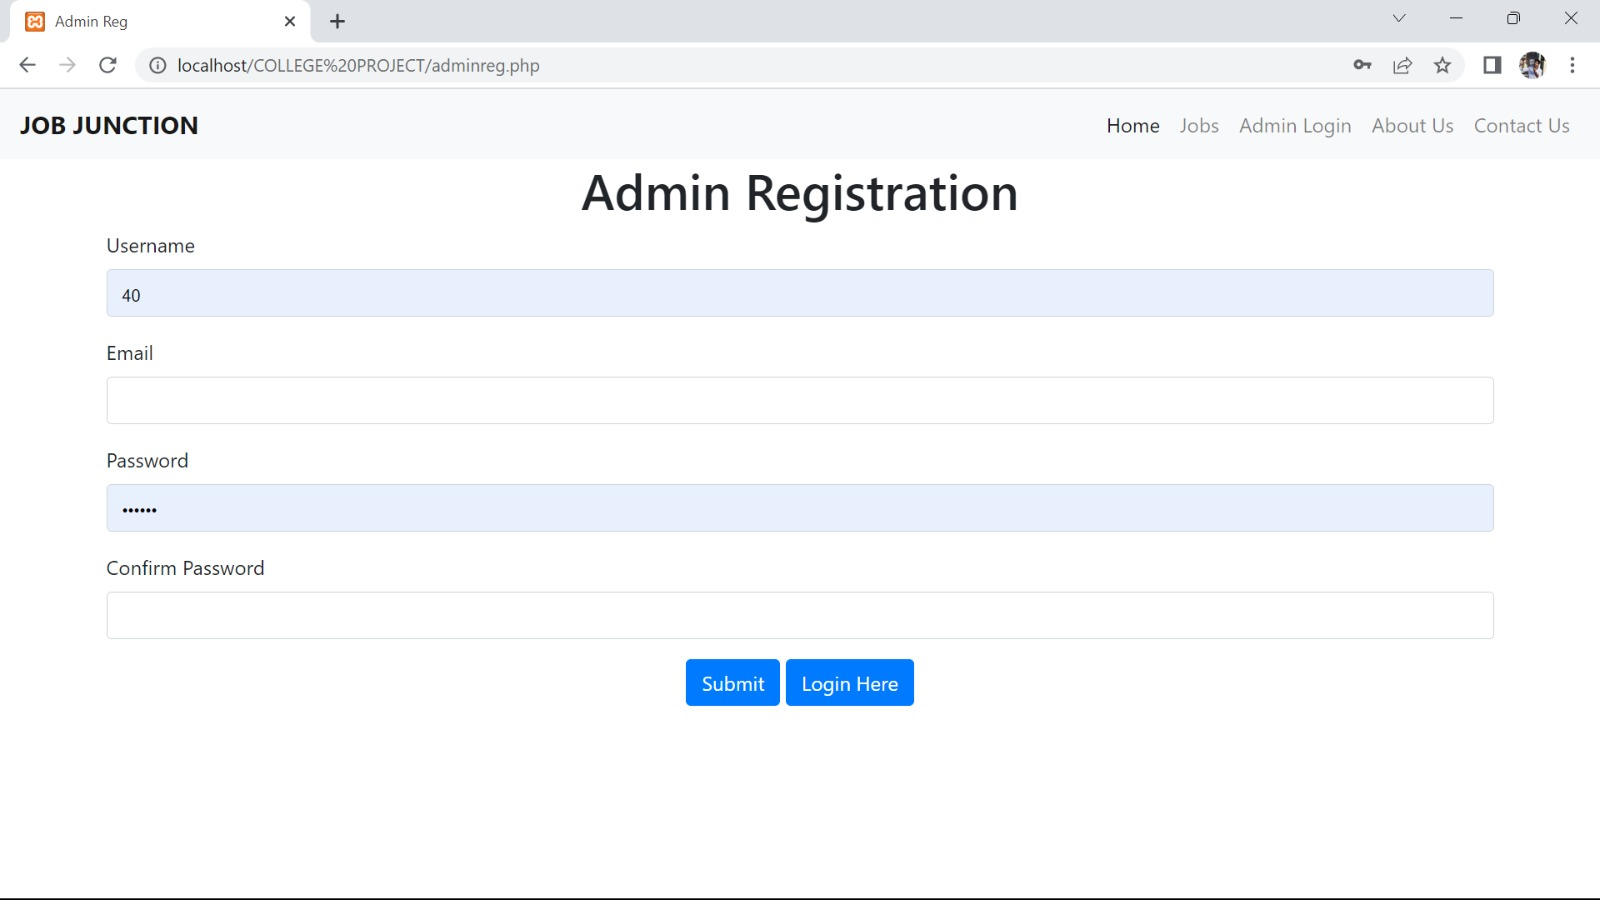
\includegraphics[width=.70\linewidth]{job1.jpeg}
	\label{fig:job1.jpeg}
\end{figure}

\section{Company Login}
Companies can login using email and password. 
\begin{figure}[h]
	\centering
	\hspace{21pt}
	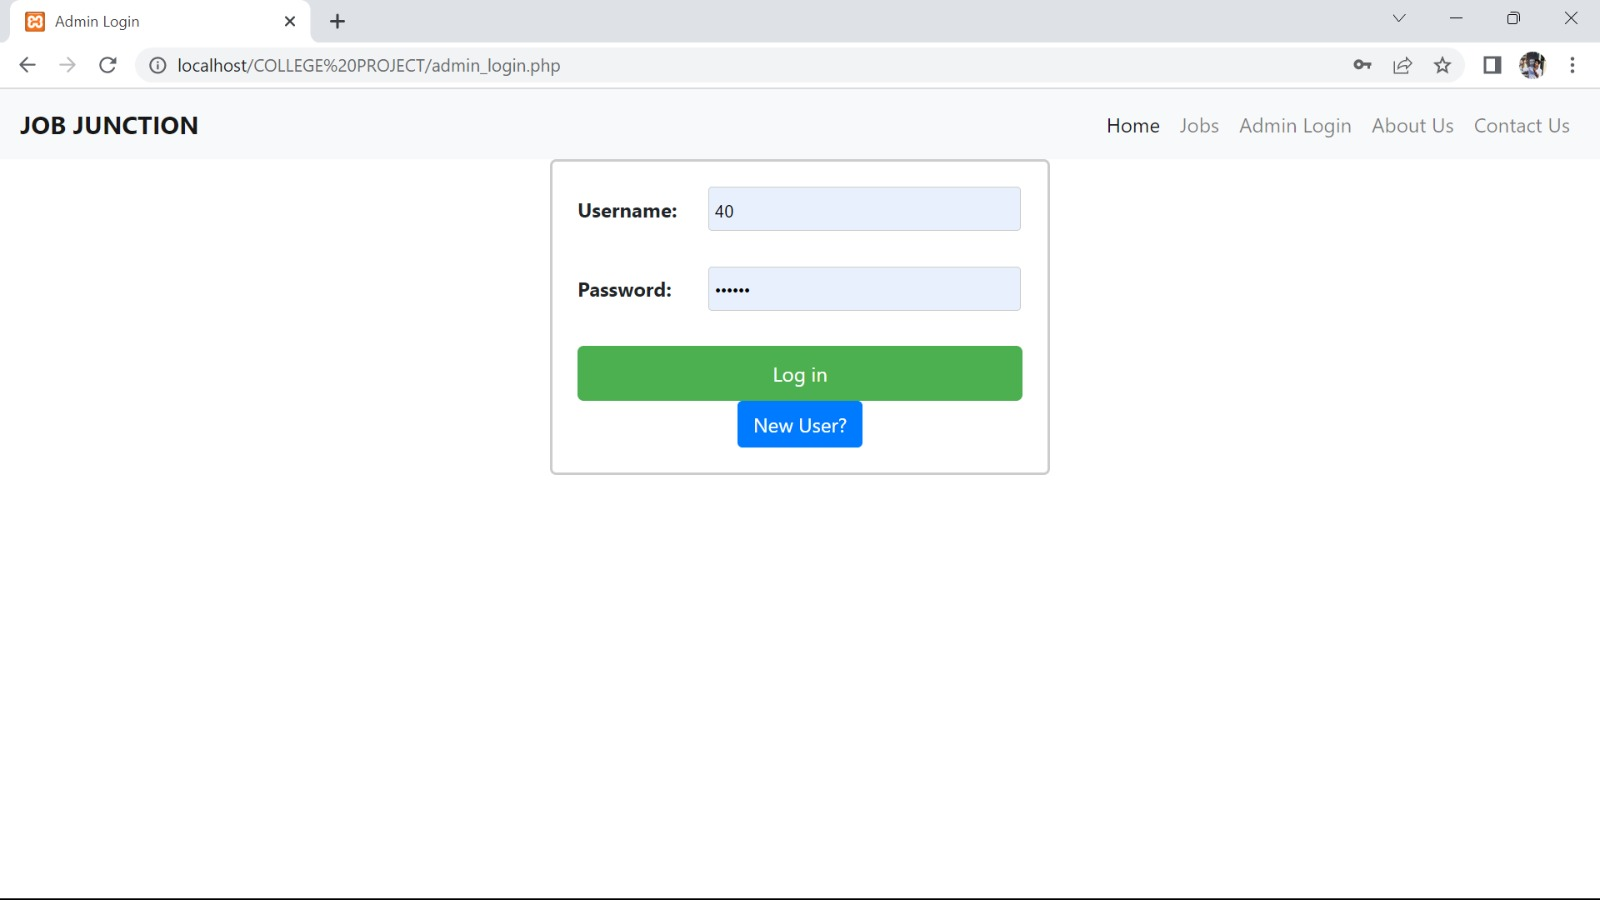
\includegraphics[width=.70\linewidth]{job3.jpeg}
	\label{fig:job3.jpeg}
\end{figure}

\section{Company Key}
In order for companies to do a recruitment, they have to purchase a key from us.
\begin{figure}[h]
	\centering
	\hspace{21pt}
	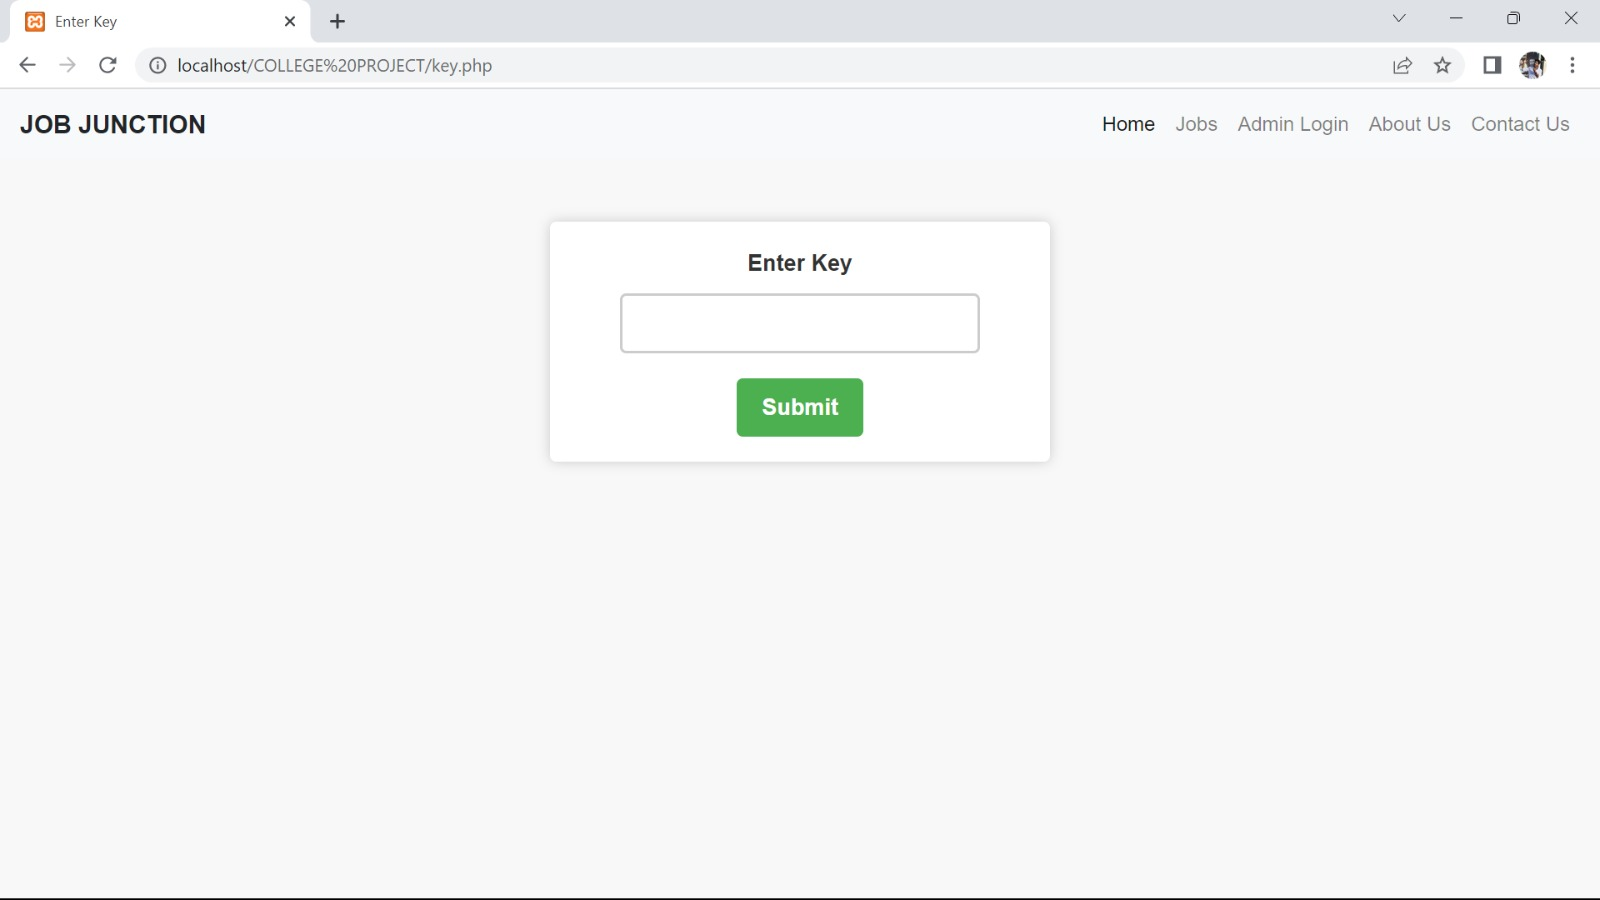
\includegraphics[width=.70\linewidth]{job2.jpeg}
	\label{fig:job2.jpeg}
\end{figure}

\section{Enter Available Jobs}
Page to enter for job recruitment.
\begin{figure}[h]
	\centering
	\hspace{21pt}
	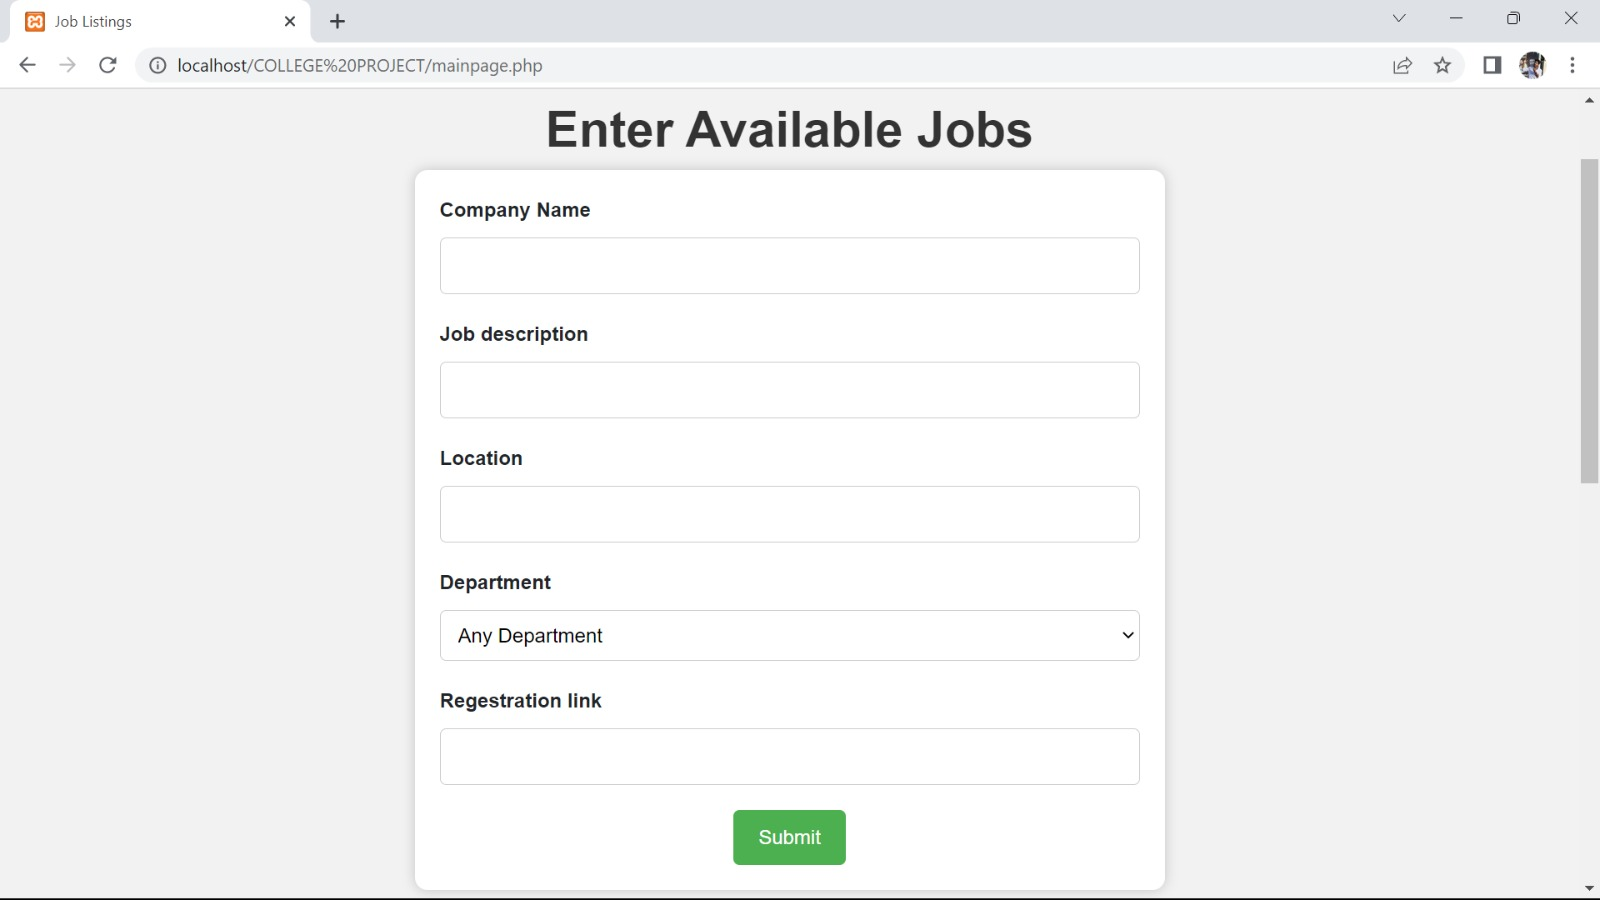
\includegraphics[width=.70\linewidth]{job0.jpeg}
	\label{fig:job0.jpeg}
\end{figure}

\section{Database}

\begin{figure}[h]
	\centering
	\hspace{21pt}
	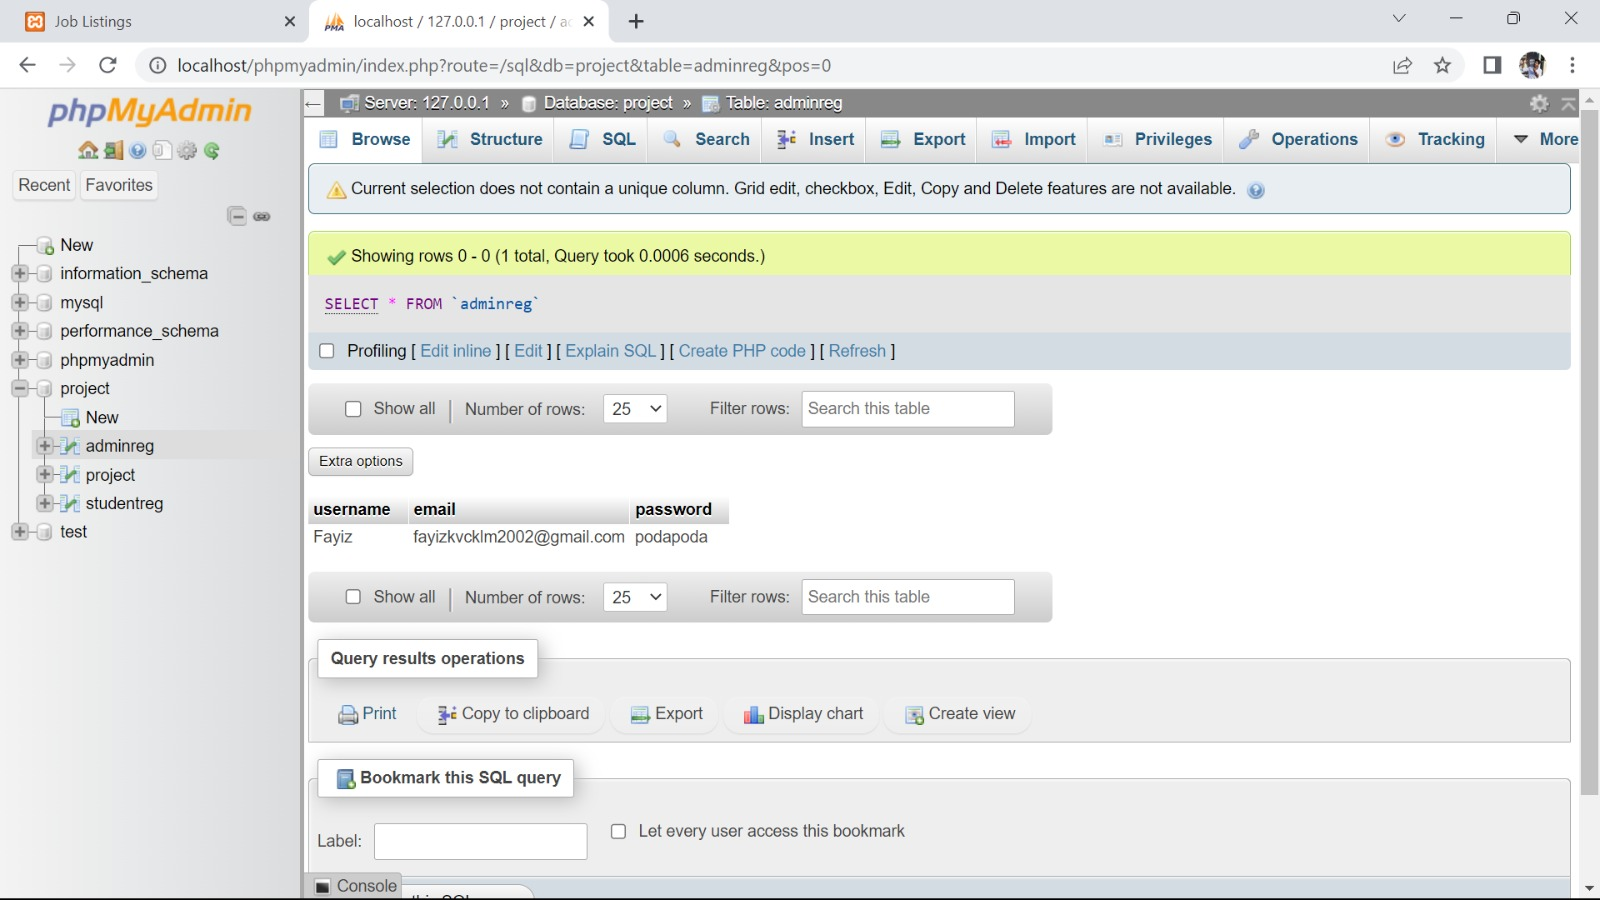
\includegraphics[width=.70\linewidth]{job7.jpeg}
	\label{fig:job7.jpeg}
\end{figure}
\begin{figure}[h]
	\centering
	\hspace{21pt}
	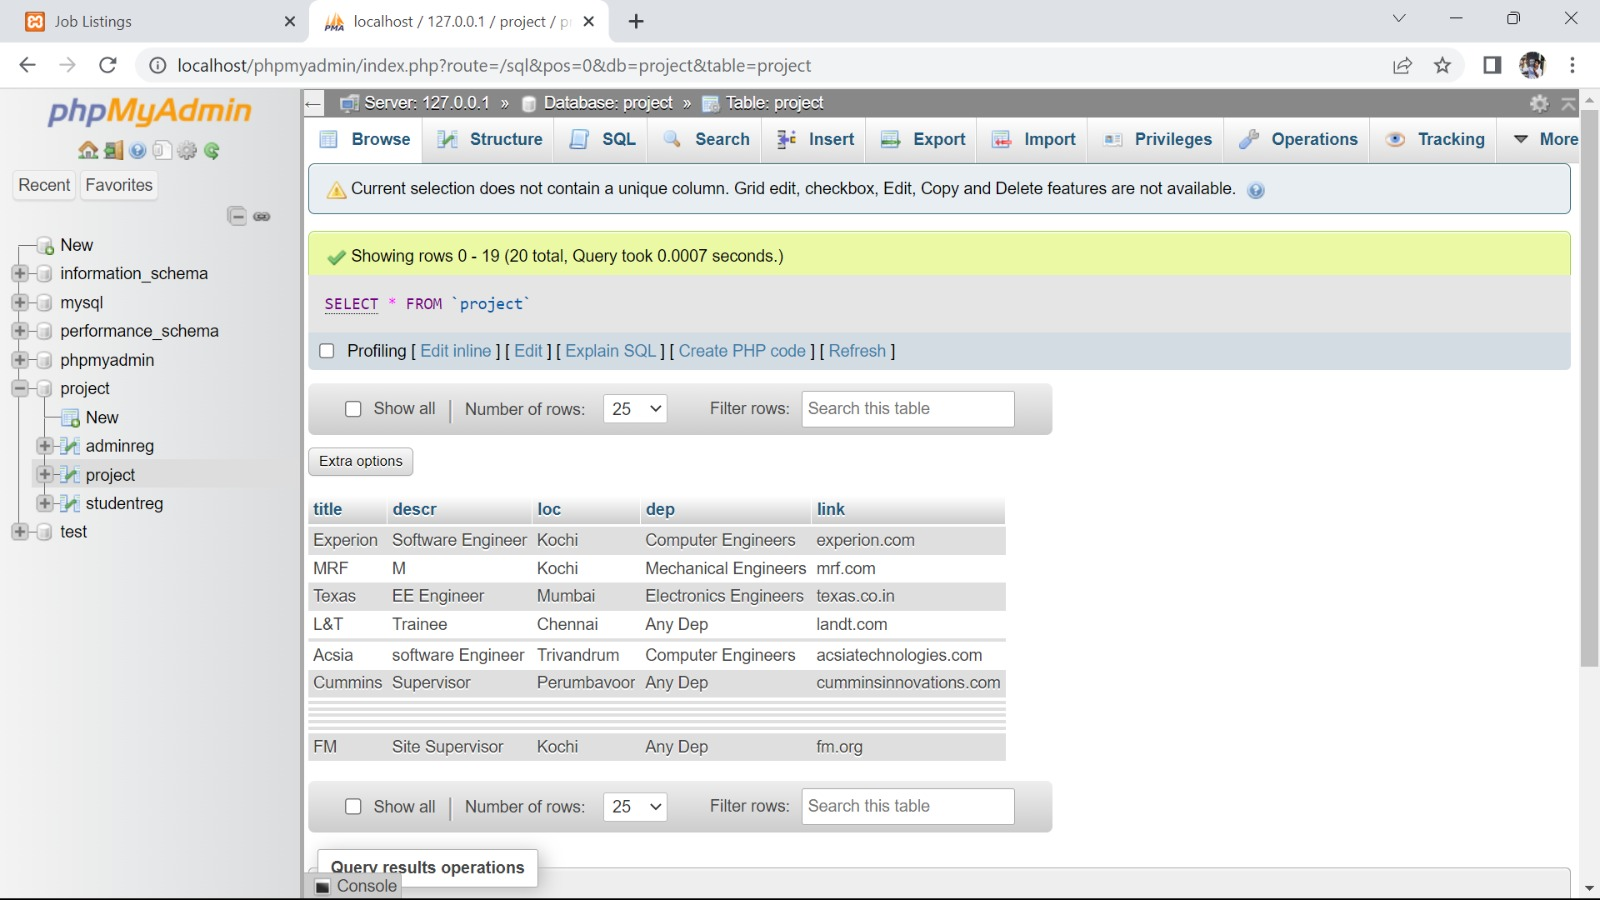
\includegraphics[width=.70\linewidth]{job8.jpeg}
	\label{fig:job8.jpeg}
\end{figure}


\chapter{Conclusion}
The Job Junction project aims to address the challenges faced by job seekers and employers in the job
search and recruitment process. By providing a comprehensive solution, Job Junction enhances the
efficiency, accessibility, and user experience of the job matching process.

Data security and privacy measures are paramount in Job Junction, with the implementation of stringent
security protocols, encryption practices, and compliance with relevant data protection regulations. This
ensures the confidentiality and integrity of user information, fostering trust and confidence among
users.

The user interface design of Job Junction prioritizes simplicity, intuitiveness, and ease of navigation.
Through user testing and feedback, the platform continuously improves its functionality, addressing pain
points and providing clear instructions to enhance the overall user experience.

Continuous improvement and feedback integration are core principles of the Job Junction project. User
feedback and behavioral data analysis are used to identify areas for enhancement, and iterative updates
are made to adapt to changing job market dynamics and user needs.
Overall, the Job Junction project strives to revolutionize the job search and recruitment process by
leveraging advanced technology, user-centric design, and effective communication. By implementing
these solutions, Job Junction aims to create a platform that benefits both job seekers and employers,
making the job search process more efficient, accessible, and successful for all parties involved.

\chapter{References}

\begin{itemize}
\item Piecework and Job Search in the Platform Economy \\
  \url{https://papers.ssrn.com/sol3/papers.cfm?abstract_id=4296733}

  \item Examining the Use of Online Platforms for Employment: A Survey of U.S. Job Seekers \\
  \url{https://dl.acm.org/doi/abs/10.1145/3411764.3445350}

  \item Online Job Search and Recruitment Platform for College Students Based on SSH \\
  \url{https://ieeexplore.ieee.org/abstract/document/9424812}
  
\end{itemize}
\end{document}
